\subsection{Analyse der generierten XML-Berichte und bestehenden Strukturen}
\label{subsec:analyse-der-generierten-xml-berichte-und-bestehenden-strukturen}

In diesem Unterkapitel wird der Aufbau der automatisch generierten Testberichte aus dem Teststand und der vorhandenen Ausgabe- und Speicherstruktur erläutert. Dies ist relevant für die Erstellung der Datenbank und das Verständnis der Ein- und Auslesefunktionen der Web-Applikation.


\subsubsection{XML-Berichtsstrukturschema}

Die vom Teststand automatisch generierten Berichte folgen einem konstanten Strukturschema, welches sich bis zu einer gewissen Ebene der XM-Struktur in jedem Bericht wiederholt. Wie im Kapitel „Grundlagen“ beschriebenen kann ein Elemente Attribute , andere Elemente und ein Inhaltswert beinhalten.

Das Stammelement heißt in allen automatisch generierten Berichten „test“ und besitzt immer das Attribut „id“. Die Zahl in diesem Attribut beschreibt die Art des \ac{DUTs}.

Das Stammelement hat die Unter- bzw. Kinderelemente „info“, „testbench, „string“ und dreimal „testmodule“. Diese Elemente haben wiederum alle weiter Unterelemente und Attribute.

Jedes der Elemente „testmodule“ hat ein Attribut „name“ durch welches Sie unterschieden werden können. Zudem hat das Element „string“ ein Namensattribut mit den Worten „test sequence status“. Der Inhalt dieses Elementes gibt an, ob der Test erfolgreich abgeschlossen wurde oder ob es ein Fehler bzw. Grenzüberschreitung eines Messwertes gab.

\begin{figure}[h]
    \centering
    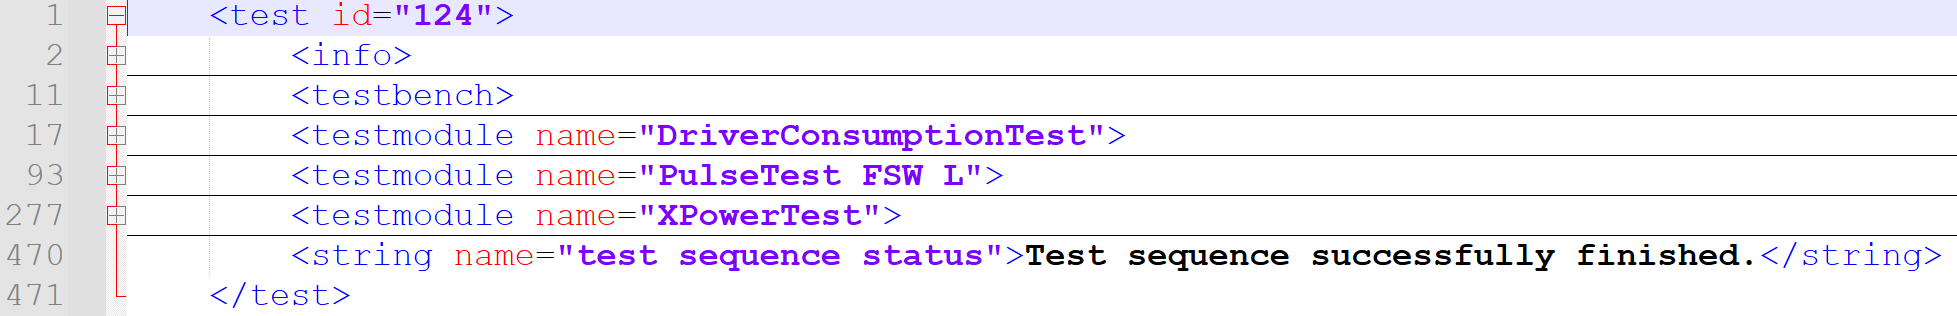
\includegraphics[width=0.8\textwidth]{Grafiken/Obere_XML-Berichtstruktur(1).png}
    \caption{Beispiel XML-berichtstruktur der Elemente nach Stammelement}
    \label{fig:3. Beispiel XML-berichtstruktur Elemente nach Stammelement}
    {Quelle: Eigene Aufnahme aus Nootpad++}
\end{figure}